\chapter{Introduction}  \label{chp_intro}
During last decades, IEEE 802.11 achieved great success in WLAN. Enormous WiFi are deployed for its high speed and simplicity of deployment. 
However, problems arise with more and more dense deployment of WiFi.
Though the throughput of WiFi has increased to x Gbit/s, the quality of experience (QoE) is not improved with the throughput.
That is because the bottleneck is located at MAC, distributed coordination function (DCF), which is the foundation of 802.11 MAC.
DCF is a random access mechanism. Details of DCF could be referred to \cite{bianchi2000performance}.

With tremendous increase of WiFi deployment, there are more and more basic service sets (BSS) overlapping with each other and each BSS has more and more devices, which will cause severe interference. 
According to Cisco Visual Network index\cite{cisco2016}, the mobile traffic will increase 53\% at CAGR within 2015-2020, which means increase eightfold during the 5 years.
What's more, other systems, like 3GPP, also engage in WLAN in the unlicensed band called LTE-U. WLAN in the unlicensed band will become more and more dense. 
Thus, supporting such a dense deployment remains critical to be solved. 

\section{Defects of Legacy 802.11}
As stated above that the bottleneck is located at MAC. It is not efficient under dense scenario.
In this section, we would display clearly about two inherent defects of legacy 802.11 MAC, including instability of DCF and unfair queueing problem.

%1. why 802.11ax, dense, DCF, contention, collision

\noindent {\Large Instability of DCF}
\vspace*{0.5cm}

Refer to Bianchi's saturated analysis of DCF\cite{bianchi2000performance}, the throughput degrades sharply with the number of stations increasing as in figure \ref{fig_thp_legacy}.
We could extend Bianchi's analysis to obtain the energy performance.
Stations have roughly three working states, "transmit", "receive" and "idle".
Check the figure \ref{fig_part_state}, with the number of stations increases, the partition of time working in transmit state for each station decreases a lot while partition in receive state increases much. 
That means a station has much less chance to transmit. And with the decrease throughput, we could know that most of transmissions are collided with others. 
Then let's look at the energy performance by checking the figure \ref{fig_eng}. 
We find that total energy consumption of a station increase a lot while successful transmissions are less.
Most of energy are wasted on listening to collided transmissions.
We thus could conclude that the DCF is inherently unstable and is not fit for dense scenario.

\vspace*{0.5cm}

\begin{figure}[!h]
\centering
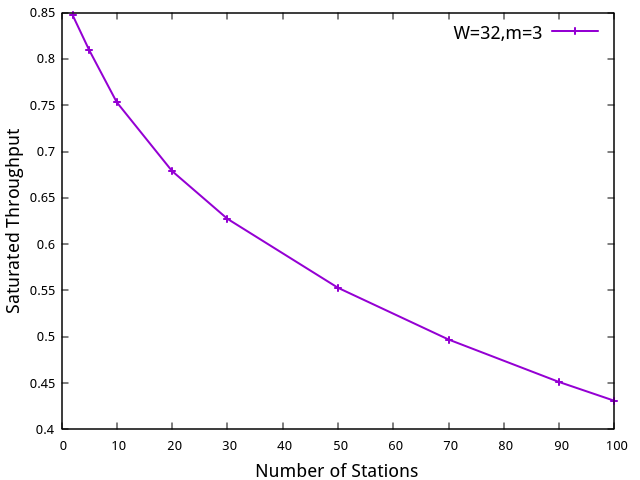
\includegraphics[scale=0.85]{./figure/chp1/n_throughput.png}
\caption{Saturated analysis: throughput vs number of stations}
\label{fig_thp_legacy}
\end{figure}
\vspace*{0.5cm}

\begin{figure}[!h]
\centering
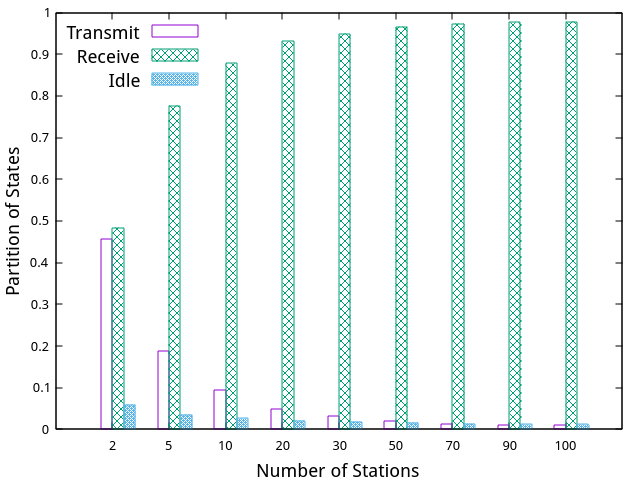
\includegraphics[scale=0.85]{./figure/chp1/n_state_partition.png}
\caption{Partition of working states of a station under saturated condition}
\label{fig_part_state}
\end{figure}

\begin{figure}[!h]
\centering
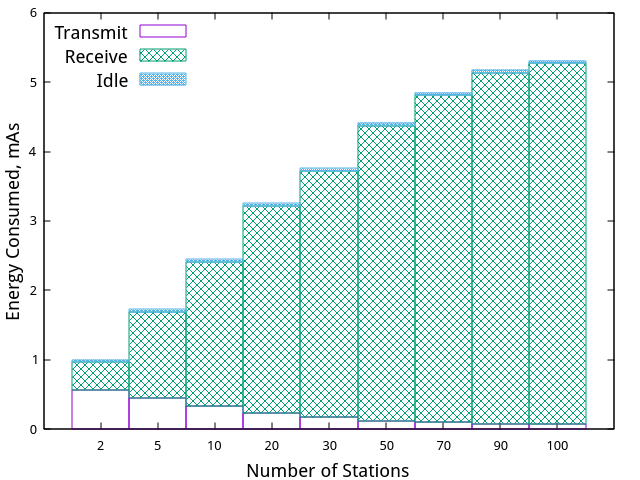
\includegraphics[scale=0.85]{./figure/chp1/n_energy_partition.png}
\caption{Energy consumption of a station under saturated condition}
\label{fig_eng}
\end{figure}

%With DCF, a random access MAC, the star topology of a 802.11 WLAN result in a absolutely unfair queueing. 
%Since in star topology,  access point (AP) needs to transmit all the down-link (DL) traffic, which is often more than $1/2$ traffic loading of the basic service set (BSS), while AP has only $1/n$ chance to access medium where $n$ is number of total stations including AP. It is, thus, an unfair queueing problem.
%What's worse, combining effect of the unstability of random access's nature and the unfair queueing problem, once under a dense scenario, the performance will degrade severely since contention and collision will occupy the channel.
%That lies the defect of legacy 802.11.
%We collectively call them dense deployment problem.
%The dense deployment problem not only degrades throughput but also waste much energy.

\noindent {\Large Unfair Queueing Problem}
\vspace*{0.5cm}
%2. ax feature, MU, central control, but OFDMA-random access

DCF together with the star topology of a BSS results in a absolutely unfair queueing. 
Check the figure \ref{fig_unfair_queueing}.
When we see the BSS with queue model, each station will be a queue, including AP.
And channel is the server, which serve packets from stations. Channel capacity determines the serve rate.
Since BSS is star topology, access point (AP) needs to transmit all the down-link (DL) traffic, which means AP shares more than 1/2 traffic loading of a BSS. 
However, since DCF is a distributed random access mechanism, AP has only $1/n$ chance to access medium where $n$ is the number of total stations including AP. It is, thus, an unfair queueing problem for up-link (UL) and DL transmission. 
This problem may not result bad consequence only if the "server" is fast enough. 
That's what a list of previous amendments, like 802.11n and ac, were doing, improving throughput from 2 Mbit/s to 7 Gbit/s. 
However, this solution doesn't resolve the unfair queueing inherently. 
The unfair queueing is always there only if each station access channel with DCF.
Once the BSS becomes congested the unfair queueing will worsen the effect of instability of DCF, resulting in more waste of spectrum and energy.
\begin{figure}[!h]
\centering
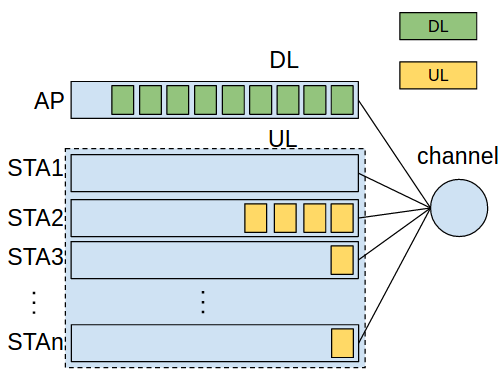
\includegraphics[scale=0.5]{./figure/chp1/unfair_queueing.png}
\caption{Unfair queueing problem of BSS}
\label{fig_unfair_queueing}
\end{figure}

\section{Solution: 802.11ax}
Previous amendments, 802.11n and 802.11ac called high throughput (HT) and very high throughput (VHT) respectively, mainly focus on modifying PHY layer to improve throughput\cite{perahia2013next}. 
However, this throughput is estimated under ideal condition, while the real world suffers a lot from instability of DCF and unfair queueing problem under dense scenario. 
That's why the QoE doesn't improve with the throughput.  
Actually, the bottleneck is located at the MAC layer.
Thus, 802.11ax task group is issued targeted at High Efficiency WLAN (HEW)\cite{802.11ax_par}, which make revolutionary modification to both MAC and PHY layers.
Only in this way, quality of experience (QoE) could be improved and energy consumption could be reduced significantly.
IEEE 802.11ax also proposes new metrics to measure the performance such as average throughput per station rather than total throughput.
Various "dense scenarios" defined in document \cite{802.11ax_simu} will be used to measure the performance of 802.11ax.
Confronting the dense deployment scenario, 802.11ax permits AP as central controller to schedule both DL and UL transmission. 
In this way, 802.11ax's MAC will not be a distributed random access mechanism and unfair queueing problem could be resolved inherently.
IEEE 802.11ax also issues multi-user (MU) PHY, which is implemented with Orthogonal Frequency Multiple Access (OFDMA) or MU-MIMO, to improve efficiency.
MU-MIMO is beyond this thesis. 
Though 802.11ax could have a scheduled MAC, random access is still high efficient in unpredictable data transmission.
Thus, a multi-channel random access is also proposed in the 802.11ax standard draft \cite{draft_ax}. 
They could be an efficient way for stations to initialize a traffic stream by sending bandwidth request.

To support OFDMA UL transmission and the OFDMA-based random access, a special control frame, trigger frame (TF), is created to implement trigger-based MU UL\cite{draft_ax}. 
Actually, the new MAC is based on DCF since it helps co-exist among BSS and other systems. The difference is that the DCF mainly works on AP which means AP needs to access channel following DCF procedure, while HE-STA (802.11ax STA) is scheduled by AP. 
Detailed illustration of 802.11ax MAC MU feature is in chapter \ref{chp_ax_feature}.

The OFDMA-based random access is the focus of this paper. 
In the following chapters, we assume a saturated condition, which means stations always have packets to transmit.
Under such assumption, we will extend Bianchi's Markov Model to model the Aloha-like OFDMA-based random access so that we could evaluate the steady state behavior of the mechanism.
At last, we propose a list of rules of configuring system parameters based on the model analysis.

\section{Related Work}
%3. related work, random acces history ? , clarify OFDMA-based random access is special
% SU/MU; aloha/CSMA; BEB/UB; saturated/unsaturated
Random access is one approach of multiaccess sharing in data network.
Inherently, collision resolution algorithms can achieve small delay with a large number of lightly loaded nodes, the stability is a major concern\cite{bertsekas1992data}\cite{chen1994medium}.  
Random access originates from Aloha and slotted Aloha in single-user channel. 
Then CSMA works as typical collision resolution  \cite{kleinrock1975packet}, which is modified and then accepted by IEEE 802.11, named CSMA/CA. 
The backoff mechanism determines the way of retransmission when failure occurs. 
Binary exponential backoff is one of typical backoff mechanism, which has been applied by 802.11 until now.
Random access has been a popular approach to MAC on unlicensed band for a long time, while cellular network  only implements random access for initial up-link access. 
With OFDMA MU channel, randomness extends from time domain to time-frequency domain, 2-dimension. 
In cellular network, IEEE 802.16 and 3GPP LTE use a multi-channel slotted Aloha.
In the literature, plenty of works focus on the multi-channel random access, and most of them work on cellular network.
\cite{choi2006multichannel} designs a 1-persistent type retransmission, i.e., no exponential backoff, to achieve a fast access.  
In \cite{zhou2008efficient}, a closed-form expression of throughput for OFDMA system is firstly given.
Many works compare performance of two backoff mechanism, binary exponential backoff and uniform backoff, like \cite{zhou2008efficient} \cite{seo2011design} \cite{kim2012performance}.
The two backoff mechanisms are implemented by IEEE 802.16 and 3GPP LTE respectively.  \cite{wei2015modeling} specifies a model estimating transient behavior of OFDMA system.
%many metrics: throughput, mean and variance of access delay, stability
All above works about OFDMA random access is an Aloha-type access in cellular network.
In addition, \cite{GeneralizedOFDMACSMACA} is one of few works for 802.11 WLAN. 
It generalizes CSMA/CA to OFDMA system for 802.11.



\section{Orgnization}
%4. our work
% the first to analyze the 802.11ax random access
Though OFDMA and multi-channel random access have been employed by IEEE 802.16 and 3GPP LTE for a long time.
It is the first time for 802.11ax to issue OFDMA and OFDMA-based random access, which is a huge evolution for 802.11.
And as far as we know, this is the first paper analyzing IEEE 802.11ax OFDMA-based random access. 
OFDMA-based random access employs binary exponential backoff and MU PHY under Trigger-based MU UL.
It is absolutely different from \cite{GeneralizedOFDMACSMACA}, since \cite{GeneralizedOFDMACSMACA} is a CSMA-like random access while OFDMA-based random access is an Aloha-like random access.
We know that \cite{bianchi2000performance} proposes an accurate Markov chain model for DCF, which is CSMA-like.
In this thesis, we show that how to extend the model to generate another Markov chain for 802.11ax to precisely depict the OFDMA-based random access.
We assume stations are under saturated condition which means their queues are never empty.
The saturated analysis is based on the key assumption of constant and independent collision probability $p$ whatever the packet is retransmitted or not.
Simulation validates our model to be accurate.
Then, we estimate the maximum system efficiency and minimum access delay. 
Since OFDMA-based random access have system parameters setting dynamically by AP, we evaluate effect of a variety of parameter sets and at last propose rules for AP to configure the parameter set. 


The thesis is organized as follows. 
More explanations of 802.11ax features are given in section \ref{sec_MU}. In section \ref{sec_RA_illu}, a detailed illustration of OFDMA-based random access procedure is presented.
Chapter \ref{chp_sys_model} contains the system model and derivation of two metrics, including system efficiency and access delay. 
Simulation which helps validate the system model is presented in this chapter.
Then chapter \ref{chp_perf_eval} is the performance evaluation of optimal performance and checks the impact of system parameters on performance.
At last rules of configuring system parameters are listed.
Chapter \ref{chp_conclu} is the conclusion remark.

%\begin{figure}
%\centering
%\includegraphics[width=0.45\textwidth]{kl}
%\caption{kl-distance}
%\label{kl}
%\end{figure}
%
%\begin{table}[t]
%\begin{center}
%\begin{tabular}{lcc}
%
%\hline
%                    &  {\small Itti's method}     & {\small Fuzzy growing}    \\
%\hline
%{\small Precision}           &  0.4475    & 0.4506 \\
%{\small Recall}              &  0.5515    & 0.5542 \\
%\hline
%
%\end{tabular}
%\caption[Evaluation of FOA sets]{\small Evaluation of FOA sets. } \label{t:FOA}
%\end{center}
%\end{table}
